\documentclass[a4paper, 12pt]{article}

% LaTeX файл с преамбулой не должен содержать команду documentclass и \begin{document}. Эти команды должны находиться только в основном документе!

\usepackage[english, russian]{babel}
\usepackage[T2A]{fontenc}
\usepackage[utf8]{inputenc}

% Cправка:

% 1) Толщина (в порядке убывания):
%   • ultra thin  |
%   • very thin   |
%   • thin        |
%   • semithick   |
%   • thick       |
%   • ultra thick |
%   • very thick  v

% 2) Цвет (способы задания):
%   • gray, red, blue, ... (см. цвета tikz в Интернете);
%   • {rgb, 255: red, 21; green, 66; blue, 128} (21/255 красного, 66/255 зелёного, 128/255 синего);
%   • red!10!blue (10% красного и (100 - 10 = 90)% синего);
%   • green!50 (зелёный с (100 - 50 = 50)% прозрачности).

% 3) Заполнение линии:
%   • loosely dashed;
%   • densely dashed;
%   • loosely dotted;
%   • densely dotted;
%   • ... (см. типы линий tikz в Интернете).

\begin{document}
    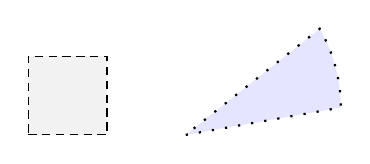
\begin{tikzpicture}
        \draw [fill = gray!10, thin, densely dashed] % densely dashed <-- штриховая линия
        (0, 0) -- (1, 0) -- (1, 1) -- (0, 1) -- cycle; % cycle <-- соединяет последнюю точку с первой

        \draw [fill = blue!10, thick, loosely dotted] % loosely dotted <-- точечная линия
        (2, 0) -- +(10:2) arc (0:30:2) -- cycle; % arc <-- дуга
        % Для arc:
        % • 0 - стартовый угол;
        % • 30 - конечный угол;
        % • 2 - радиус дуги.
        % (10:2):
        % • 10 - угол в градусах (в радианах: 10rad);
        % • 2 - радиус.
        % В пути можно указывать координаты относительно последней точки, используя +(...)
        % Для лучшей мобильности рисунка в путях рекомендуется использовать относительные координаты с cycle в конце
        % (тогда для перемещения нужно поменять координаты только стартовой точки, а не всех)
        % Если требуется переместить перо, чтобы оно при этом не рисовало, надо в пути вместо -- использовать ++
    \end{tikzpicture}
\end{document}